\begin{nestedsection}{Evaluation, Results and Discussion}{evaluation}
	To evaluate the performance of R4, we compare it with state-of-the-art systems that provide the capability of performing background reasoning on semantic streaming data.
	These include Etalis \citep{EP-SPARQL}, Sparkwave \citep{sparkwave}, Streaming knowledge bases \citep{walavalkar08streamingkb}, and the incremental reasoner presented in \citep{inc-reasoning-background-knowledge}.
	To the best of our knowledge, the latter two implementations were never made public, so we compare R4 against Etalis and Sparkwave only.
	The experiments are performed on an Intel Core i5 computer with 3.2 GHz and 8 GB memory.
	We set up Jtalis (the Java wrapper of Etalis) over SWI-Prolog v7.2.1 and installed Sparkwave v0.5.1.

	\begin{nestedsection}{Motivating Case}{evaluation: motivating case}
		We first used a 1.1 million triple real-world dataset from the SemSorGrid4Env project that contains weather observations over a period of ten days.
		Inspired by a query in \citep{SRBench}, we formulated a rule that entails that a given observation is of a weather pattern classified as a hurricane if it is of a wind speed that exceeds that of a previously classified hurricane;
		it also entails that the wind speed observed exceeds that of a given historically recorded hurricane (\reffig{SRBench-rule}).
		\begin{figure*}
			\centering
			\begin{verbatim}
Forall ?obs ?sensor ?result ?value ?v ?hur ?hurWind (
    If And( ?obs [ssn:observedProperty -> wind_speed]
    		?obs [ssn:observedBy -> ?sensor]
            ?obs [ssn:observationResult -> ?result] 
            ?result [ssn:hasValue -> ?value]
            ?value [ssnExt:hasQuantityValue -> ?v]
            ?hur [rdf:type -> yago:Hurricane111467018]
            ?hur [dbpprop:1MinWinds -> ?hurWind] 
            External (pred:numeric-greater-than(?v ?hurWind)) )
    Then ?obs [ssn:observedWeatherType -> yago:Hurricane111467018] )
			\end{verbatim}
			\caption{The RIF-Core rule inspired by SRBench.}
			\labelfig{SRBench-rule}
		\end{figure*}
		This rule involves dealing with static data regarding past hurricanes, dynamic data regarding ongoing sensor readings, and also needs to perform reasoning against an ontology of background knowledge to identify the hurricanes that are instances of the specified class of hurricanes.
		For the historical hurricane data, we prepared a small dataset taken from dbpedia, containing information about a number of hurricanes.

		The experiment consisted of pushing the whole stream to the compiled R4 system and measuring the time taken to process all the data, repeated for a variety the window ranges.
		We ran this rule successfully on R4 and Jtalis getting correct results.
		However, Sparkwave was unable to read the dataset correctly as it does not parse blank nodes;
		this is because it uses the hash-join algorithm to improve time efficiency, as we show in \refsec{evaluation: comparative results}, but builds the hashtables based on the URIs of the incoming data.
	\end{nestedsection}
	\begin{nestedsection}{Comparative Results}{evaluation: comparative results}
		In order to compare the efficiency of R4 against both Etalis \emph{and} Sparkwave, we formulated a second experiment using the synthetic dataset from the Berlin SPARQL Benchmark \citep{BSBMresults} which was used in the Sparkwave paper.
		We generated a 1.1 million triples dataset containing information about 100,000 limited-time offers made available by some online marketplace.
		We used a small schema that has 329 product types arranged in a 4-level hierarchy.

		The rule we chose to express in each system, shown in \reffig{BSBM-rule}, entails the offer price for all products that are on offer.
		As offers may be associated with product super-types, background reasoning is needed to determine the offer price for specific product sub-types.
		\begin{figure*}
			\centering
			\begin{verbatim}
Forall ?offer ?product ?vendor ?price ?from ?to ?delivery ?webpage(
    If And( ?offer [rdf:type -> bsbm_voc:Offer]
            ?offer [bsbm_voc:product -> ?product]
            ?offer [bsbm_voc:vendor -> ?vendor]
            ?offer [bsbm_voc:price -> ?price]
            ?offer [bsbm_voc:validFrom -> ?from]
            ?offer [bsbm_voc:validTo -> ?to]
            ?offer [bsbm_voc:deliveryDays -> ?delivery]
            ?offer [bsbm_voc:offerWebpage -> ?webpage]
            ?offer [dc:publisher -> ?publisher]
            ?offer [dcc:date -> ?date] )
    Then ?product [bsbm_voc:offerPrice -> ?price] )
			\end{verbatim}
			\caption{The RIF-Core rule inspired by the Berlin SPARQL benchmark.}
			\labelfig{BSBM-rule}
		\end{figure*}

		Before we move on to more detailed analysis of the results, we noticed that this rule takes significantly longer to process in Etalis (3 hours for the 1.1 million dataset with 1 second time window compared to ${<10}$ minutes for the other two systems).
		However, when we changed the `And' into a series of `seq's, the system runs 20x times faster (7.5 minutes for the same test).
		Such a drastic difference is likely to be caused by the optimisation of Etalis for the \emph{seq} operator: being intended for \emph{event processing} rather than continuous querying/reasoning, the order of arrival of triples is often more relevant than their simple coincidence in the system.
		In order to present results that provide a meaningful comparison between the time efficiency of each system with regards to changing window ranges, as in \reffig{all-systems-varying-windows}, we chose to modify the rule when evaluating ETALIS to use \emph{seq} instead of \emph{And}.
		It should be noted that we recognise that this modified rule is not semantically equivalent to that by which we evaluate R4 and Sparkwave, which cannot express the \emph{seq} operator, but is sufficient to contrast the effect of window range on the time- and memory-efficiency of the three systems.
		\begin{figure}
			\centering
			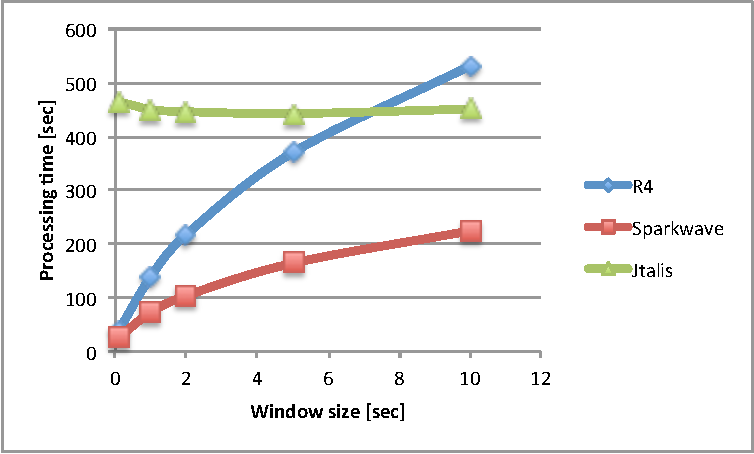
\includegraphics[width=0.45\textwidth]{all-systems-varying-windows}
			\caption{A comparison of the times taken by the systems R4, Sparkwave and ETALIS to process 1.1 million triples from a single input stream, given sliding windows of various ranges over the input stream.}
			\labelfig{all-systems-varying-windows}
		\end{figure}

		As shown in \reffig{all-systems-varying-windows}, R4 is faster than Etalis for small sliding windows but slower than Sparkwave, and, while the time-to-complete increases with window range in both Sparkwave and R4, that of Etalis appears to remain fairly constant for the sliding-window ranges tested.
		The growing difference between R4 and Sparkwave as the range of the sliding windows increases is likely due to the fact that Sparkwave uses a hash join algorithm with garbage-collection window-maintenance while the current implementation of R4 uses loop joins over lists maintained by indexing over timestamps;
		as data remains valid for longer, the beta memories (i.e valid windows) grow bigger, and window-joins in R4 need significantly longer to iteratively check for matches compared to the hash-based look-up of those in Sparkwave.
		More time-efficient, multi-index window-joins are to be considered for R4 in future work.

		We also examined the memory consumption of R4, Sparkwave, and Jtalis throughout a run.
		Setting the sliding window range to five seconds, \reffig{all-systems-memory-consumption} shows the amount of memory used by the three engines during the life time of the BSBM rule.
		It shows that, while R4 and Jtalis follow similar patterns, Sparkwave memory needs are significantly higher.
		Though we cannot know the reason for this without a thorough inspection of the Sparkwave code-base, we suspect that this is related to the manual garbage collection performed.
		\begin{figure}
			\centering
			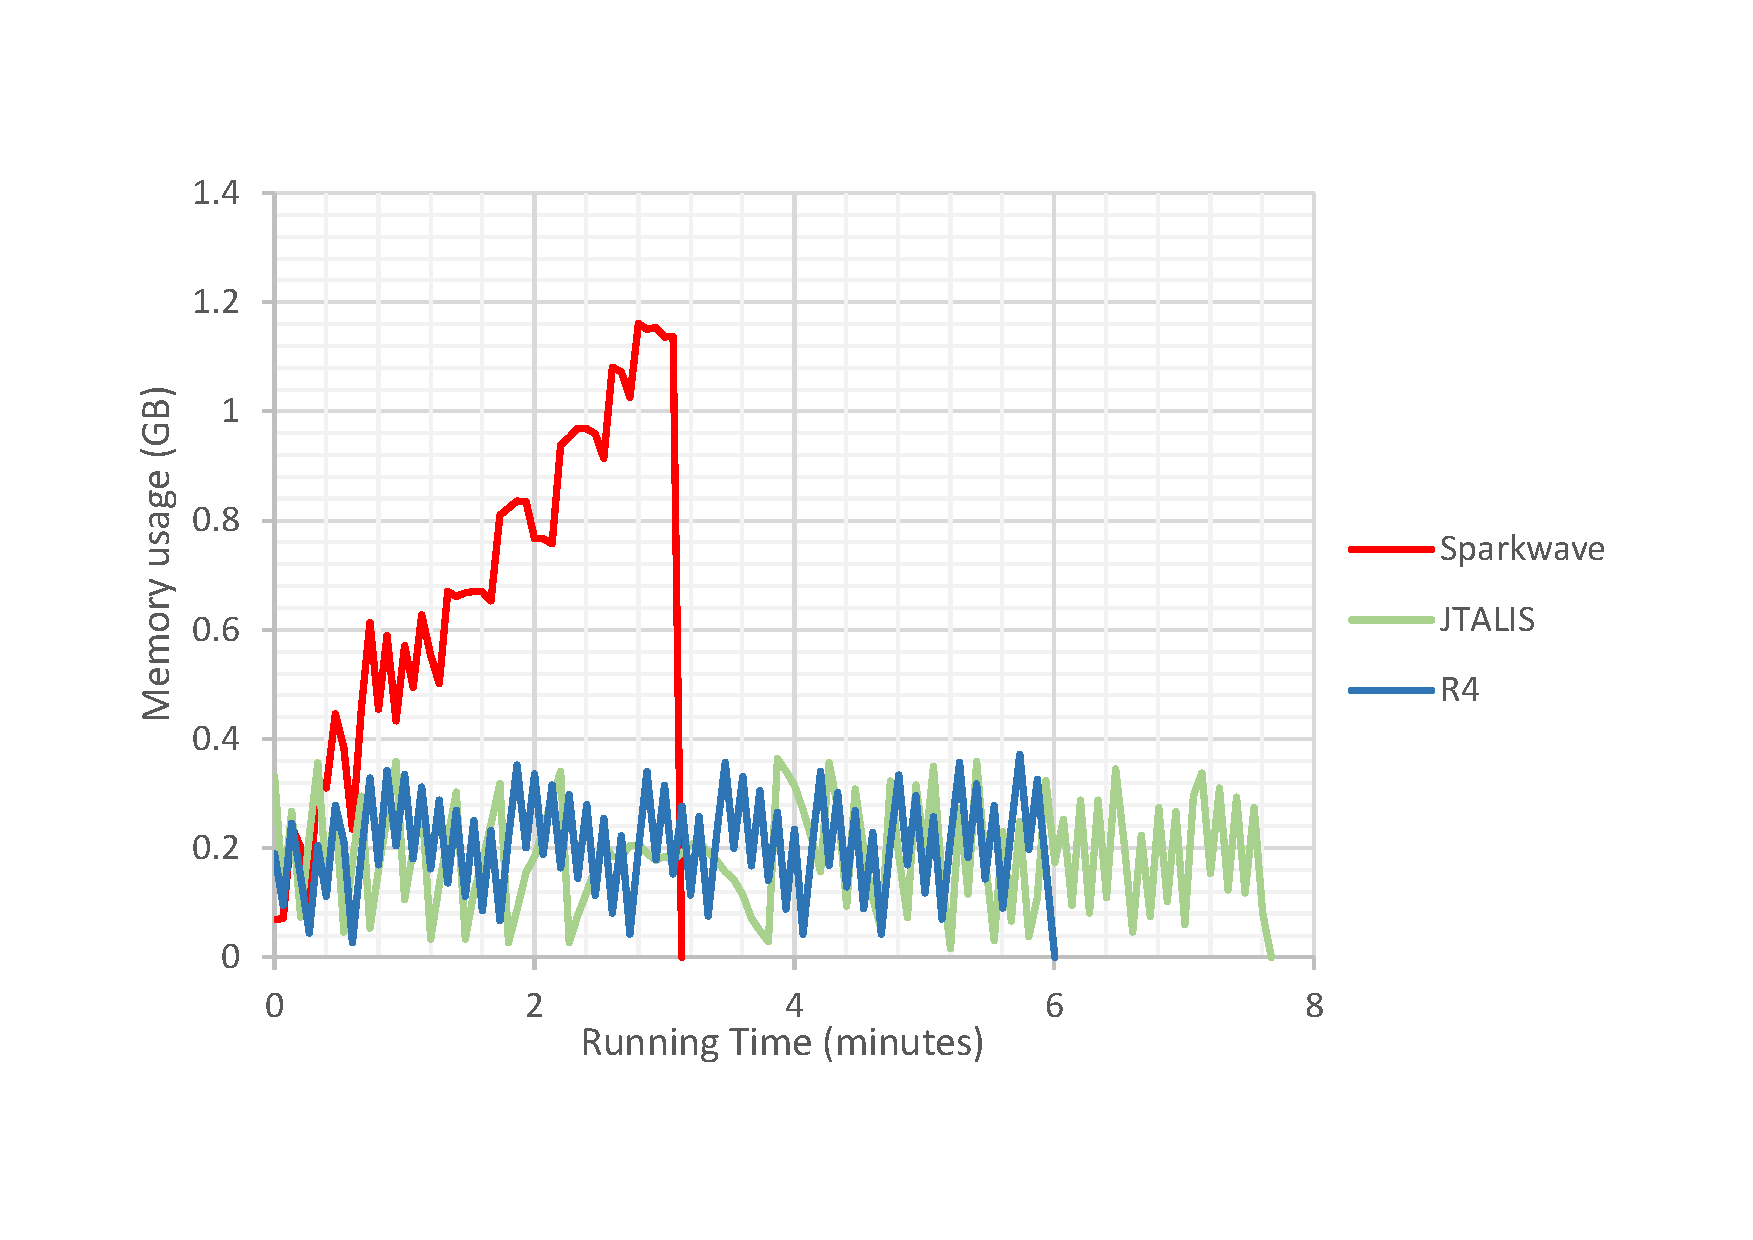
\includegraphics[width=0.5\textwidth]{memoryConsumptionComparison}
			\caption{A comparison of the memory consumed by the systems R4, Sparkwave and ETALIS throughout a run processing 1.1 million triples from a single input stream, given sliding windows of 10 seconds over the input stream.}
			\labelfig{all-systems-memory-consumption}
		\end{figure}
	\end{nestedsection}

%	\subimport{conclusions/}{future-work.tex}
\end{nestedsection}
